\section{Participant Learning Experiment}
\label{sec:results:participantlearning}

\begin{figure}[t]
  \centering
  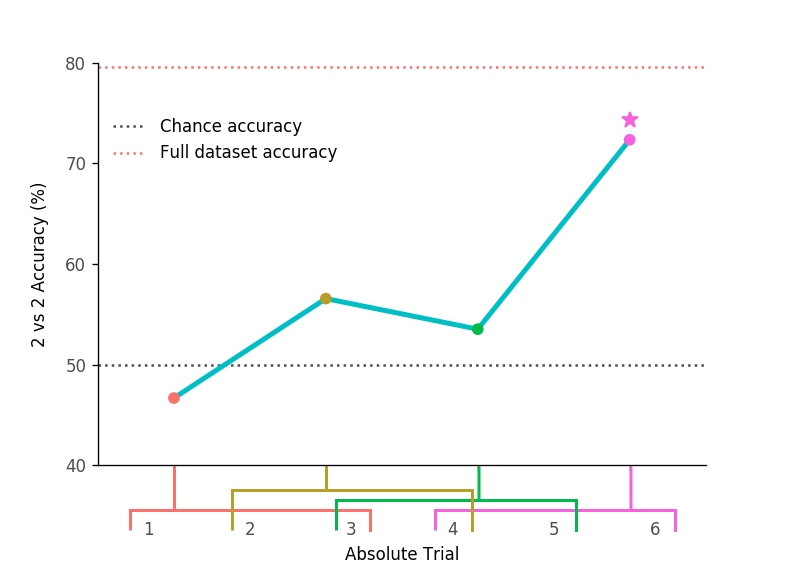
\includegraphics[width=0.75\linewidth]{figures/learning}
  \caption[\tvt Accuracy over Trials]{
    A graph of 2 vs 2 accuracy over trials in the 0 - 700 ms time period. This 
    graphic shows how participant learning develops over time with a sliding 
    window of three trial averages.  2 vs 2 accuracy increases notably in the 
    last window, showing learning occurs in the later half of trials. A star 
    indicates a statistically significant value with $p < 0.001$ (FDR 
    corrected). This figure courtesy of Chad C. Williams.
  }
  \label{fig:learning}
\end{figure}

This experiment builds on the Semantic Representation Experiment, and aims to 
identify the trial at which we can detect meaning. To do this we utilize a 
sliding window with a window size of three trials over our included dataset.   
Figure~\ref{fig:learning} plots the \tvt accuracy over trials using this 
sliding window technique for the 0 - 700 ms time period. When we average 
exposures (1, 2, 3) of each symbol, we achieve a \tvt accuracy of 
\textbf{46.70\%}.  Exposures (4, 5, 6) produce an accuracy of \textbf{72.35\%} 
with $p < 0.001$ (FDR corrected). We see a similar pattern in the 0 - 500 ms 
time period with accuracies of 55.87\%, 56.27\%, 58.53\%, and 64.86\% for each 
sliding window respectively. We applied bootstrapping to generate normal theory 
confidence intervals for both the first and last sliding window, which 
confirmed with $p < 0.05$ that there is a statistically significant difference 
in \tvt accuracy between the first trials participants see (1, 2, 3) and the 
later trials participants see (4, 5, 6).

Due to a reduction in data, the \tvt accuracy over trials (4, 5, 6) is slightly 
lower than the \tvt accuracy in the previous experiment, which used trials 
beyond the 6th exposure. However, this result confirms we can detect 
participant learning with our model. This is a novel and unqiue way to analyze 
the process of learning an artificial language mapping, which has benefits that 
will be further discussed in Section~\ref{sec:results:participantlearning}.
